\section{What do groups look like?}
\begin{questions}
	\question In the rectangle puzzle, what actions were the generators? What other actions are there besides the generators?
	\begin{solution}
		\par Horizontal flip and vertical flip
		\par Other actions are the `do nothing' and the `horizontal followed by the vertical flip'
	\end{solution}
	
	\question In the light switch puzzle, what actions were the generators? What other actions are there besides the generators?
	\begin{solution}
		\par See previous exercice
	\end{solution}
	
	\question Can an arrow in a Cayley diagrem ever connect a node to itself?
	\begin{solution}
		\par Yes, the `do nothing' action.
	\end{solution}

	\question Exercices 1.1 of Chapter 1 defined a group. Create its Cayley diagram using the technique from this chapter.
	\begin{solution}
		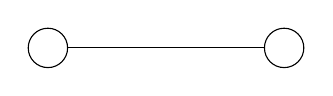
\begin{tikzpicture}
			\draw (0,0) -- (3,0);
			\draw[fill=white] (3,0) circle (0.25cm);
			\draw[fill=white] (0,0) circle (0.25cm);
		\end{tikzpicture}
	\end{solution}
	
	\question Exercise 1.4 of Chapter 1 defined a group. Create its Cayley diagram using the technique from this chapter.
	\begin{solution}
		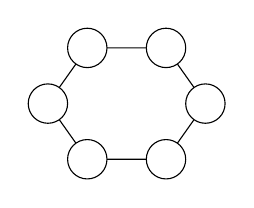
\begin{tikzpicture}
			\draw (0.5,0.707) -- (1,0) -- (0.5,-0.707) -- (-0.5,-0.707) -- (-1,0) -- (-0.5,0.707) --cycle;
			\draw[fill=white] (1,0) circle (0.25cm);
			\draw[fill=white] (0.5,0.707) circle (0.25cm);
			\draw[fill=white] (0.5,-0.707) circle (0.25cm);
			\draw[fill=white] (-0.5,0.707) circle (0.25cm);
			\draw[fill=white] (-0.5,-0.707) circle (0.25cm);
			\draw[fill=white] (-1,0) circle (0.25cm);
		\end{tikzpicture}
	\end{solution}

	\question Exercise 1.13 describes an infinite group which can be generated with just one generator. Can you draw an infinite Cayley diagram for it? (Just draw a portion of the diagram that makes the infinite pattern clear)
	\par How does that Cayley diagram compare to one for the group in Exercise 1.14 part (a)?
	
	\question Exercise 1.14 part (d) described a two-element group. Can you draw a Cayley diagram for it? Which arrow or arrows should you use and why?
	\begin{solution}
		\par $1 \leftrightarrow -1$ en op beide element een pijl naar zichzelf voor de actie `$\cdot 1$'.
	\end{solution}

	\question Section 2.2 introduced the rectangle puzzle. Imagine instead a square puzzle with its corners labeled the same way. Such a puzzle would allow a new move that was not possible with the rectangle puzzle, you could rotate a quarter-turn clockwise.
	\begin{parts}
		\part Make the map of this group
		\begin{solution}
			Zie $D_4$
		\end{solution}

		\part Why is the quarter-turn move not `allowed' in the rectangle puzzle?
		\begin{solution}
			Zie later
		\end{solution}
	\end{parts}
	
	\question Most groups can be generated may different ways, and each way gives rise to a corresponding way to connect a Cayley diagram with arrows. For example, consider the group $V_4$, which we met in the rectangle puzzle. Let's shorten the names of its actions to $n, h, v$ and $b$, meaning (respectively) no action, horizontal flip, vertical flip, and both (a horizontal flip followed by a vertical flip).
	\par We sam that $h$ and $v$ together generate $V_4$. But it is also true that $h$ and $b$ together would generate $V_4$, or $v$ an $b$ together. (You can verify these facts by exploring the rectangle realm using these generators on your own numbered rectangle.)
	\begin{parts}
		\part Make a copy of Figure 2.9 and add to it a new type of arrow, representing the action $b$.
		\begin{solution}
			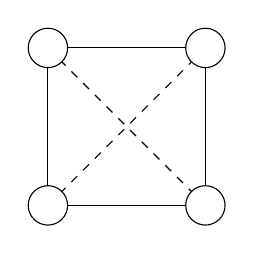
\begin{tikzpicture}
				\draw (0,0) -- (2,0) -- (2,2) -- (0,2) -- cycle;
				\draw[dashed] (0,0) -- (2,2);
				\draw[dashed] (0,2) -- (2,0);
				\draw[fill=white] (0,0) circle (0.25cm);
				\draw[fill=white] (0,2) circle (0.25cm);
				\draw[fill=white] (2,2) circle (0.25cm);
				\draw[fill=white] (2,0) circle (0.25cm);
			\end{tikzpicture}
		\end{solution}

		\part Make a copy of your answer  to part (a), with the arrows representing $h$ removed. How does your diagram show that $v$ and $b$ are sufficient to generate $V_4$?
		\begin{solution}
			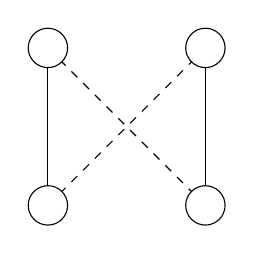
\begin{tikzpicture}
				\draw (2,0) -- (2,2);
				\draw (0,0) -- (0,2);
				\draw[dashed] (0,0) -- (2,2);
				\draw[dashed] (0,2) -- (2,0);
				\draw[fill=white] (0,0) circle (0.25cm);
				\draw[fill=white] (0,2) circle (0.25cm);
				\draw[fill=white] (2,2) circle (0.25cm);
				\draw[fill=white] (2,0) circle (0.25cm);
			\end{tikzpicture}
			\par It is still possible to reach each situation.
		\end{solution}
		
		\part Make a copy of your answer to part (a)n, with the arrows representing $v$ removed. How does your diagram show that $h$ and $b$ are sufficient to generate $V_4$?
		\begin{solution}
			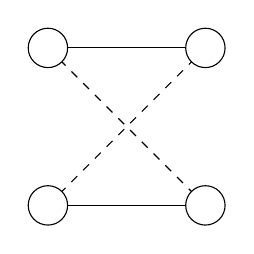
\begin{tikzpicture}
				\draw (0,0) -- (2,0);
				\draw (0,2) -- (2,2);
				\draw[dashed] (0,0) -- (2,2);
				\draw[dashed] (0,2) -- (2,0);
				\draw[fill=white] (0,0) circle (0.25cm);
				\draw[fill=white] (0,2) circle (0.25cm);
				\draw[fill=white] (2,2) circle (0.25cm);
				\draw[fill=white] (2,0) circle (0.25cm);
			\end{tikzpicture}
			\par It is still possible to reach each situation.
		\end{solution}
	\end{parts}

	\question If you've done all the exercises to this point, you've encountered two different Cayley diagrams that have the two-node form shown here.
	\par Can you come up with another group whose Cayley diagram has this form?
	
	\question If you've done all the exercices to this point, you've encountered two different Cayley diagrams that have the four-node form shown here.
	\par Can you come up with another group whose Cayley diagram has this form?
	
	\question We have not yet seen a group whose Cayley diagram has the three-node form called $C_3$, shown in the top left of Figure 2.10. Can you come up with a group whose Cayley diagram has that form?
	
	\question A group's generators have a special status in a Cayley diagram for the group. What is that special status?
	\begin{solution}
		Represented by the arrows.
	\end{solution}
	
	\question Chapter 1 required groups to satisfy Rule 1.5, which states, ``There is a predefined list of actions that never changes.'' How does this rule impact the appearance of Cayley diagrams? (Or how would diagrams be different if this rule were not a requirement?)
	\begin{solution}
		If a action would not be executed on a certain node.
	\end{solution}
	
	\question Chapter 1 required groups to satisfy Rule 1.6, which states, ``Every action is reversible.'' What constraint does this place on the arrows in a Cayley diagram? Can you draw a diagram that does not fit this constraint? (That is, draw a diagram that almost deservers the name ``Cayley diagram'', except for that one rule violation.)
	\begin{solution}
		Every node should have an arrow departing and arriving.
	\end{solution}

	\question Chapter 1 required groups to satisfy Rule 1.7, which states, ``Every action is deterministic.'' What constraint does this place on the arrows in a Cayley diagram? Can you draw a diagram that does not fit this constraint? (That is, draw a diagram that almost deserves the name ``Cayley diagram,'' except for that one rule violation.)
	\begin{solution}
		An arrow departing from a node can only arrive in one node.
	\end{solution}
	
	\question Chapter 1 required groups to satisfy Rule 1.8, which states, ``Any sequence of consecutive actions is also an action.'' How do we depend upon this fact when using a Cayley diagram as a map?
	\begin{solution}
		One should be able to reach every node by executing consecutive actions.
	\end{solution}
	
	\question If we created a equilateral triangle puzzle, like the square puzzle in exercise 2.8, what would the valid moves be? Map the group of such a puzzle.
	\begin{solution}
		\par Flip with respect to any symmetry axis. (Three flips) And a rotation over 60\textdegree, 120\textdegree and 180\textdegree. 
		\par This forms $D_3$.
		\par It has 2 generating actions, one flip and one rotation.
	\end{solution}

	\question A regular $n$-gon is a polygon with $n$ equal sieds an $n$ equal angles. You have already analyzed regular $n$-gons with $n=3$. (equilateral triangle, Exercise 2.18) and $n=4$ (square, Exercise 2.18).
	\begin{parts}
		\part Based on what you know about the cases $n=3$ and $n=3$, make a conjecture about how many actions will be in the group of a regular $n$-gon for any $n>2$.
		\begin{solution}
			There are $n$ axes of symmetry and $n$ rotations of 360\textdegree$:n$. This results in $2n$ symmetries.
		\end{solution}
		
		\part Test your conjecture by making te map of the group for a regular pentagon ($n=5$).
		\begin{solution}
			$D_5$ has 10 symmetries.
		\end{solution}
	\end{parts}
\end{questions}